
\documentclass{beamer}
\usetheme{Singapore}
\usecolortheme[dark,accent=blue]{solarized}
\setbeamertemplate{navigation symbols}{\insertframenumber}
\setbeamercolor{navigation symbols}{fg = solarizedAccent}
\setbeamerfont{navigation symbols}{size = \tiny}

\usepackage{hyperref, tikz}
\usetikzlibrary{arrows.meta, shapes.geometric}
\tikzset{>={To[length=3mm,width=3mm]}}

\title{Winning baseball games by\\solving statistics puzzles}
\author{Scott Powers}
\date{JHU ECE Seminar\\September 18, 2025}
\begin{document}

  \begin{frame}
      \maketitle
      \vfill\hfill
\includegraphics[width = 4cm]{../../assets/rice_logo_white.png}
  \end{frame}

  \begin{frame}{Books about Baseball Teams Using Analytics to Win}
    \begin{columns}
      \begin{column}{0.25\textwidth}
        \centering
        
\includegraphics[width = \textwidth]{images/books/moneyball.jpg}\\
        ~\\
        2002\\ Oakland\\ Athletics
      \end{column}
      \begin{column}{0.25\textwidth}
        \centering
        
\includegraphics[width = \textwidth]{images/books/the_extra_two.jpg}\\
        ~\\
        2008\\ Tampa Bay\\ Rays
      \end{column}
      \begin{column}{0.25\textwidth}
        \centering
        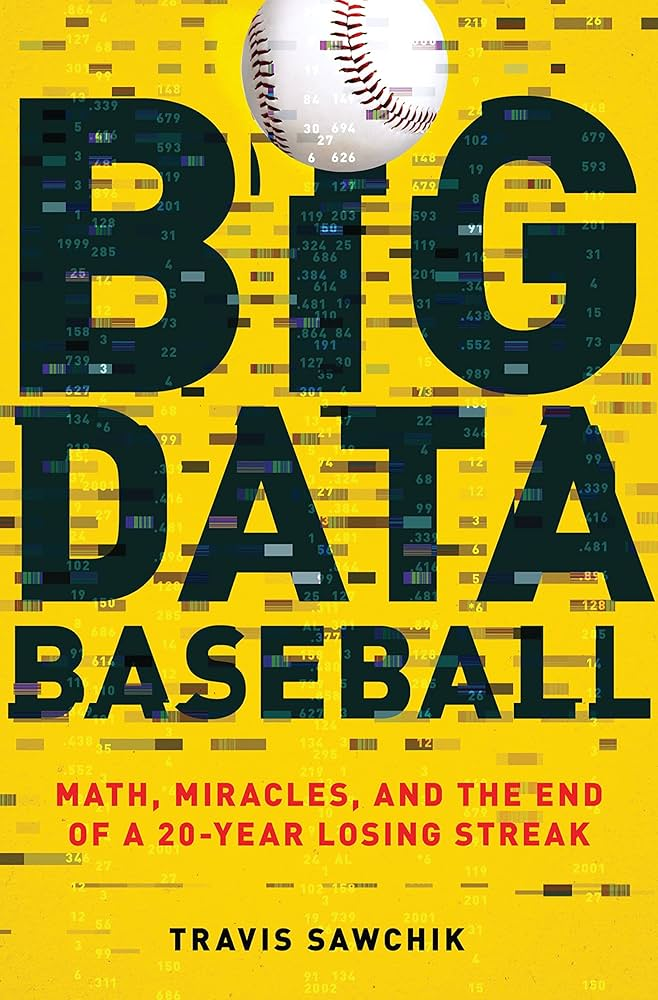
\includegraphics[width = \textwidth]{images/books/big_data_baseball.jpg}\\
        ~\\
        2013\\ Pittsburgh\\ Pirates
      \end{column}
      \begin{column}{0.25\textwidth}
        \centering
        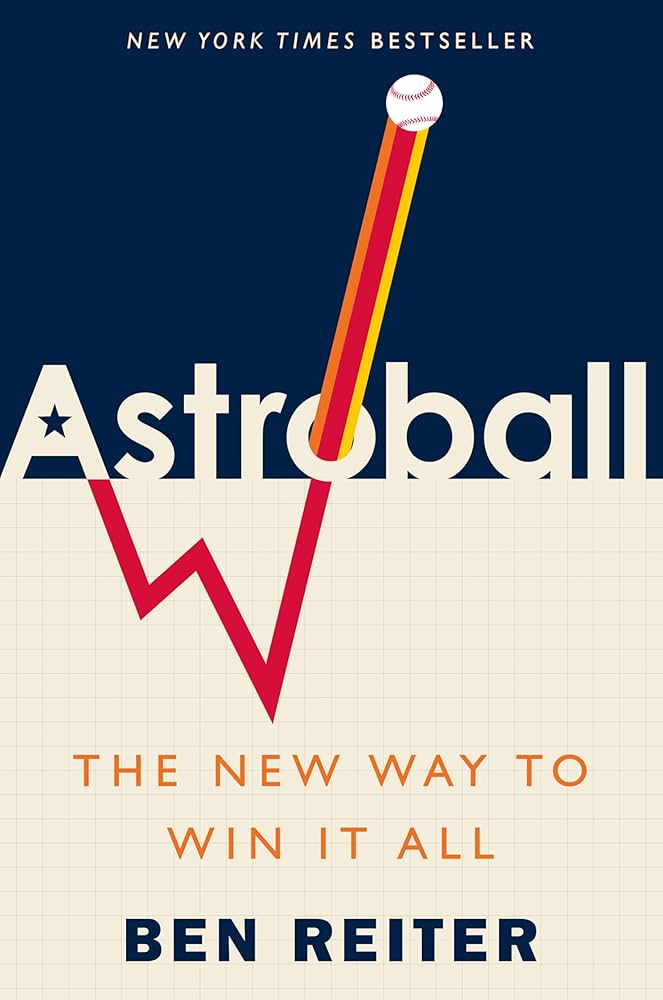
\includegraphics[width = \textwidth]{images/books/astroball.jpg}\\
        ~\\
        2017\\ Houston\\ Astros
      \end{column}
    \end{columns}
  \end{frame}

  \begin{frame}{MLB R\&D Staff Sizes (according to Reddit)}
    \begin{columns}
      \begin{column}{0.55\textwidth}
        \centering
        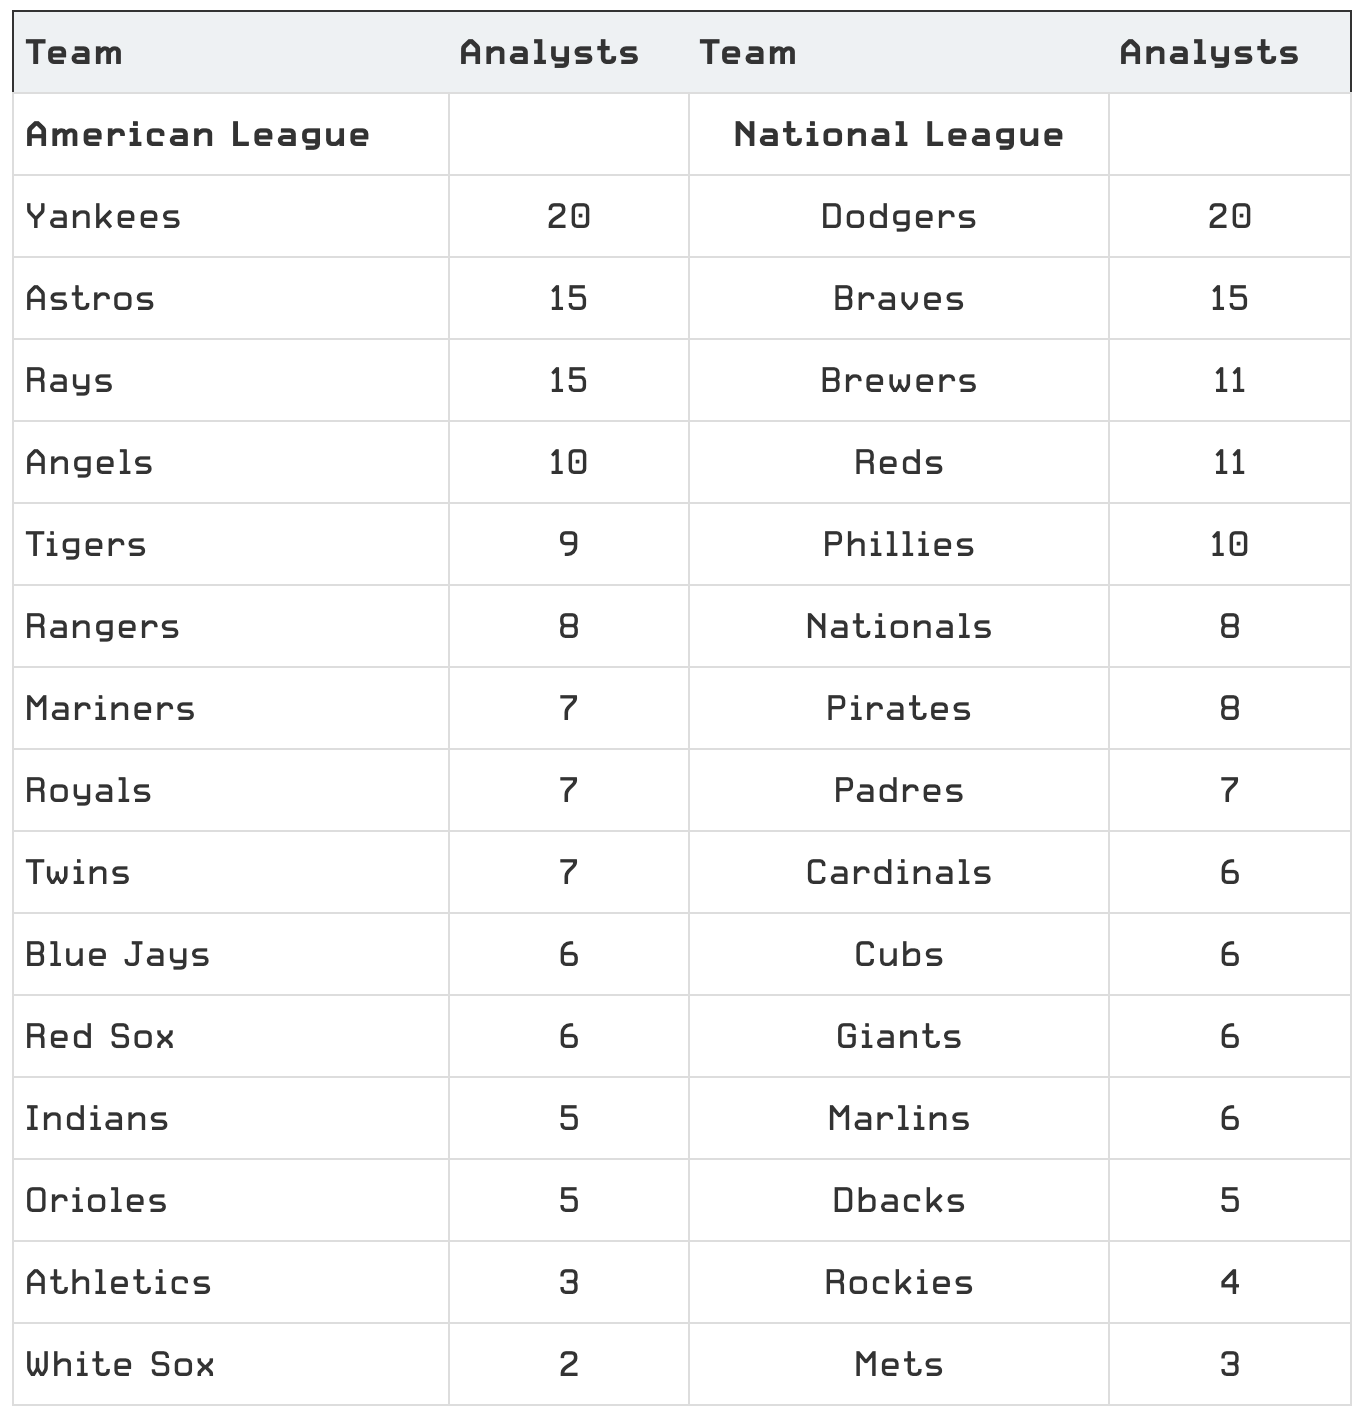
\includegraphics[width=\textwidth]{images/staff_2018.png}\\
        2018
      \end{column}
      \begin{column}{0.45\textwidth}
        \centering
        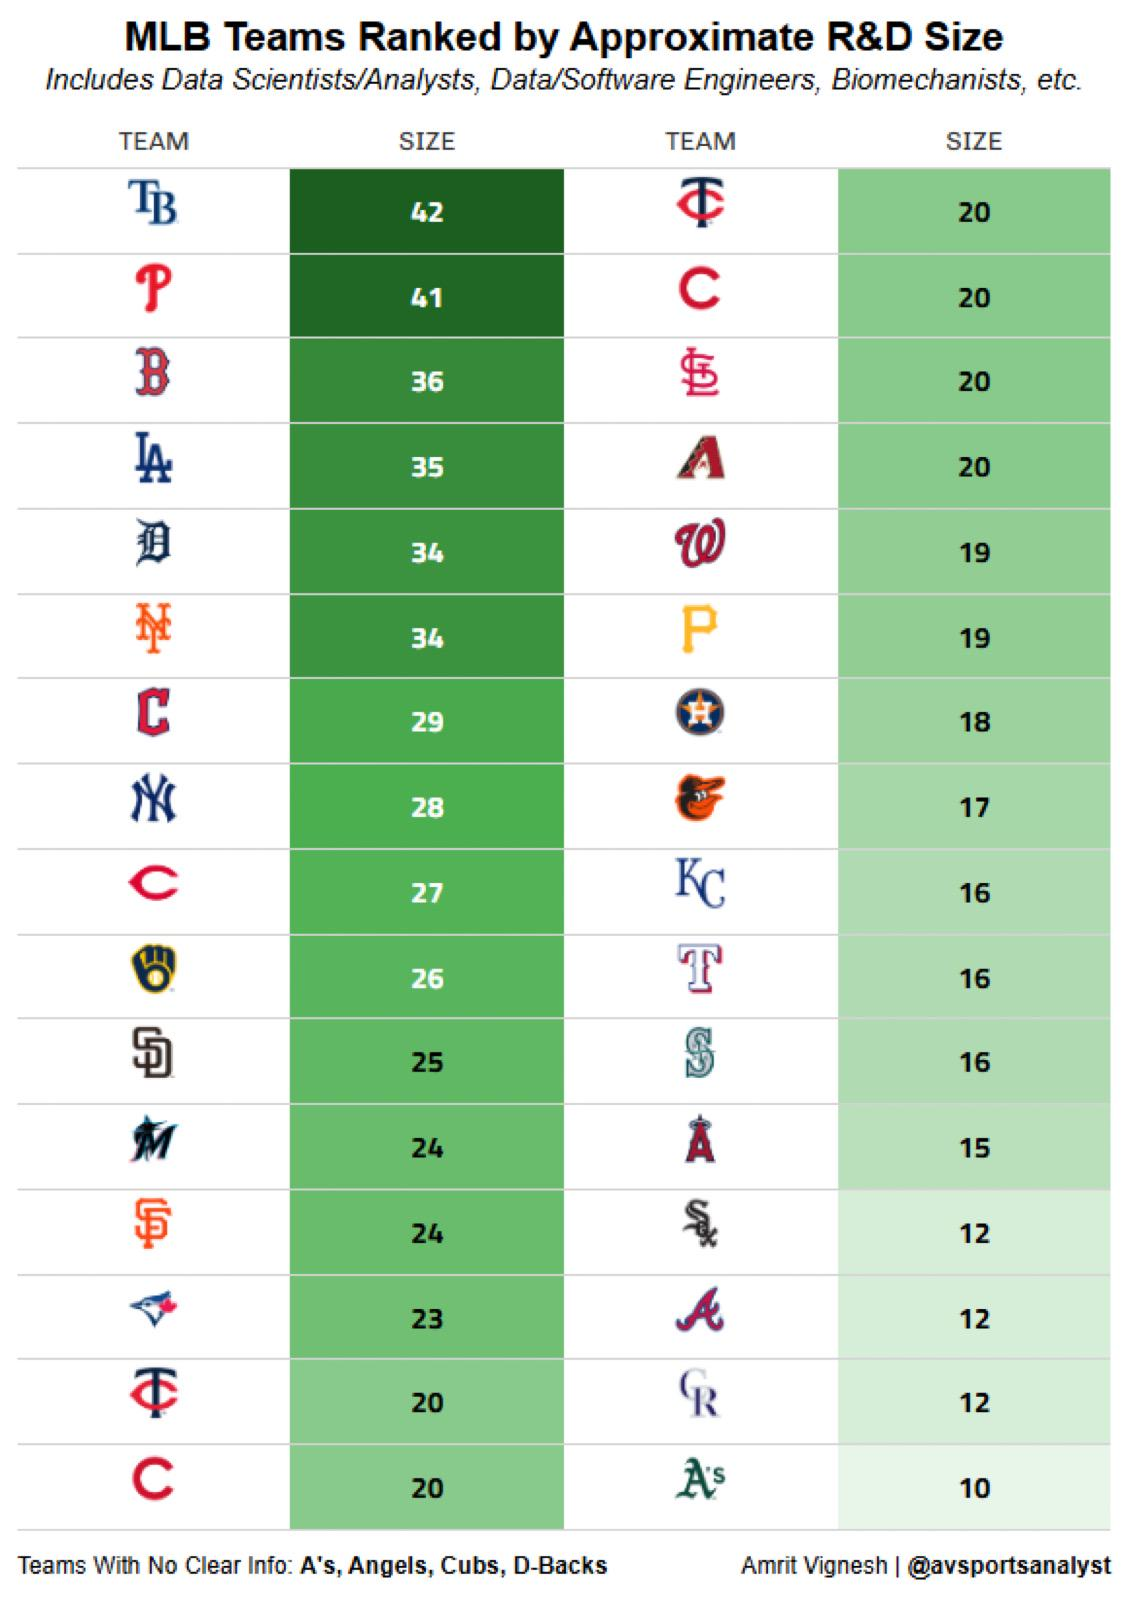
\includegraphics[width=\textwidth]{images/staff_2025.jpeg}\\
        2025
      \end{column}
    \end{columns}
  \end{frame}

  \begin{frame}{What are they all doing?}
    \centering
    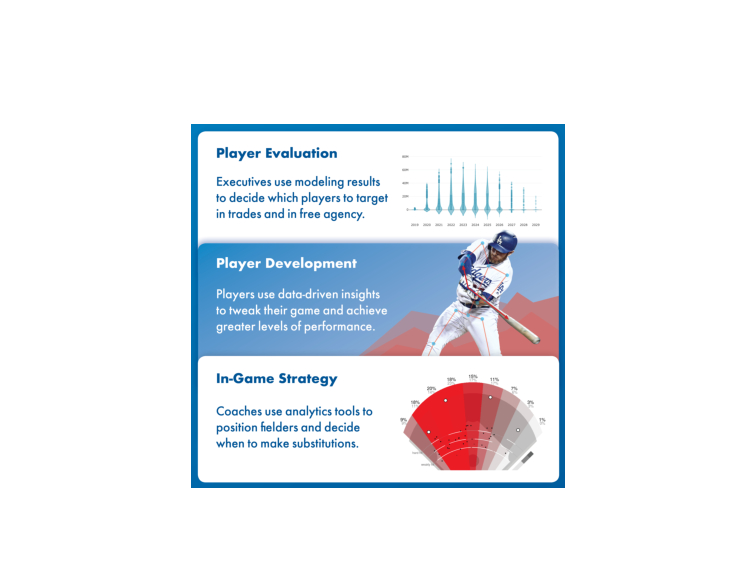
\includegraphics[height=0.8\textheight]{images/applications.pdf}
  \end{frame}
  
  \begin{frame}{Three Puzzles}
    \begin{columns}
      \begin{column}{0.46\textwidth}
        \begin{enumerate}
          \item[I:] Runner-pitcher strategy\\ under pickoff limits
          \vspace{1.5cm}
          \item[II:] Pitcher evaluation from\\ pitch tracking
          \vspace{1.5cm}
          \item[III:] Inference from swing-level\\ bat tracking
        \end{enumerate}
      \end{column}
      \begin{column}{0.4\textwidth}
        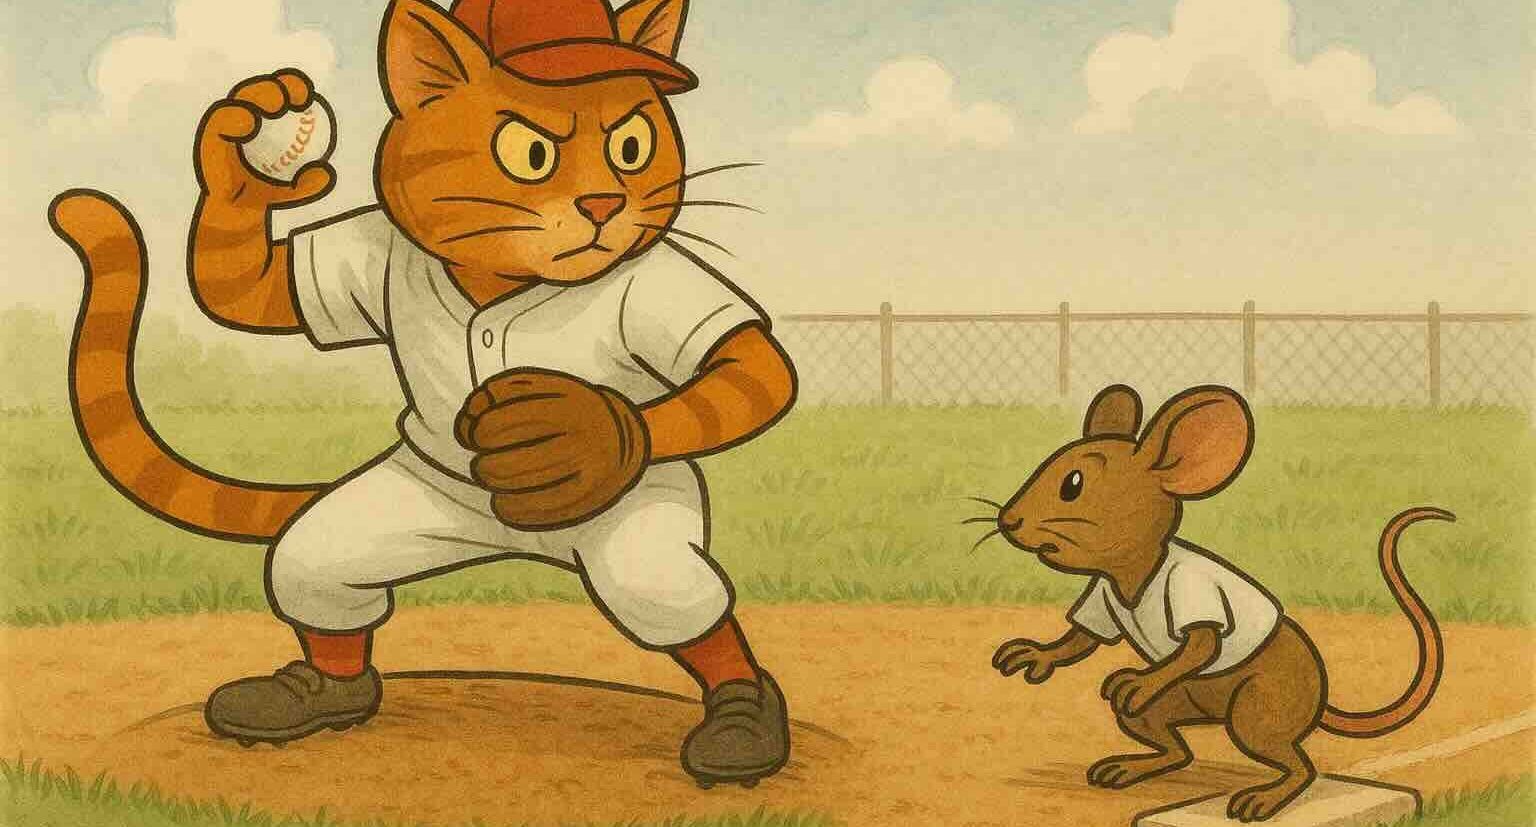
\includegraphics[width = \textwidth]{images/cat_and_mouse.jpg}\\
        ~\\
        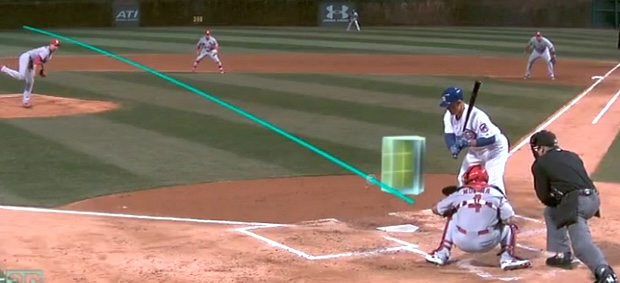
\includegraphics[width = \textwidth]{images/pitch_tracking.jpg}\\
        ~\\
        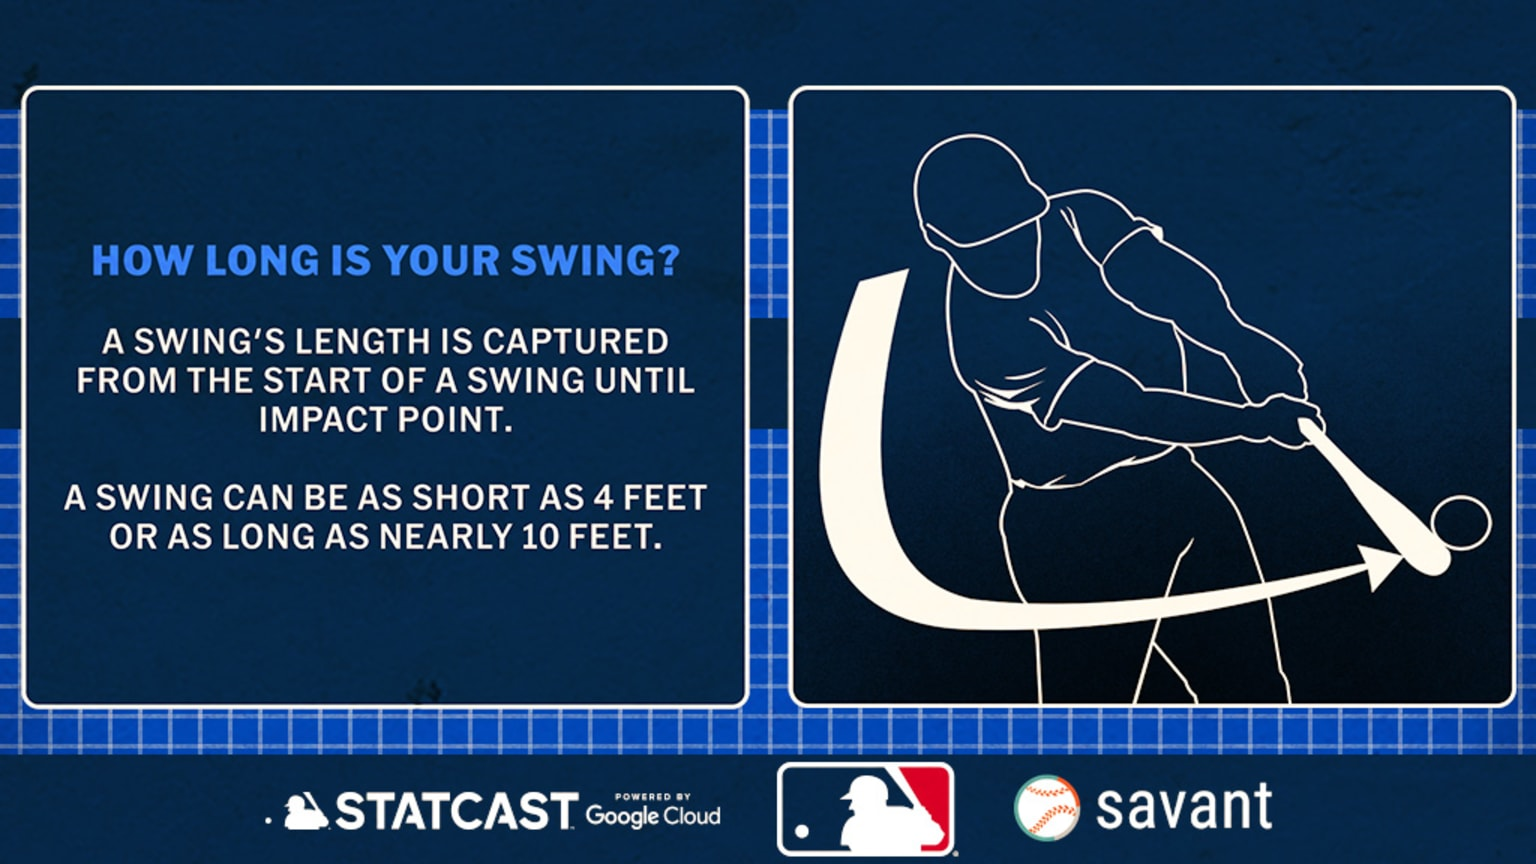
\includegraphics[width = \textwidth]{images/swing_length.jpg}
      \end{column}
    \end{columns}
  \end{frame}

  \begin{frame}
    \Large Part I: Runner-pitcher strategy under pickoff limits\normalsize\\
    \vfill
    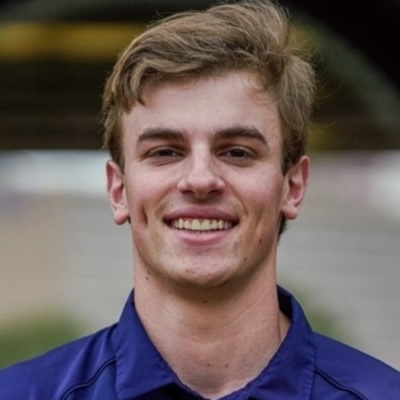
\includegraphics[height=0.5in]{images/collaborators/hahn.jpg}
    \alert{Jacob Hahn}, Rice University $\rightarrow$ Chicago Cubs\\
    ~\\
    
\includegraphics[height=0.5in]{images/collaborators/ramani.jpg}
    \alert{Sivaramakrishnan Ramani}, Rice University\\
    ~\\
    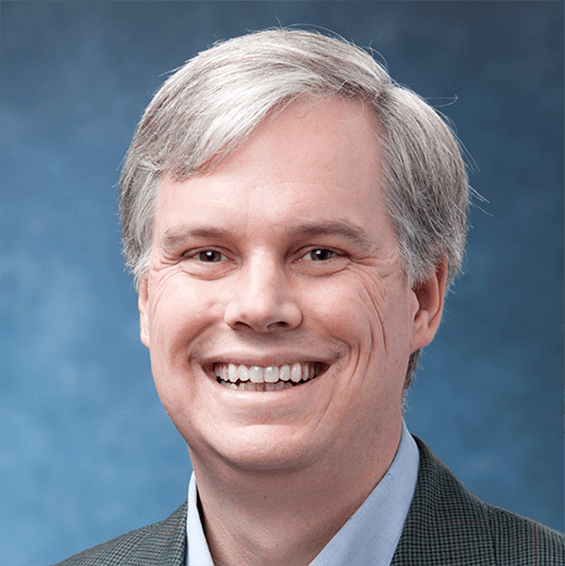
\includegraphics[height=0.5in]{images/collaborators/schaefer.png}
    \alert{Andrew Schaefer}, Rice University\\
    ~\\
    Working paper:\\
    \small Hahn J, Powers S, Ramani S, Schaefer A ``The Two-Foot Rule: A game theoretic analysis of the pickoff limit in Major League Baseball''
  \end{frame}

  \begin{frame}{Background}
    \centering
    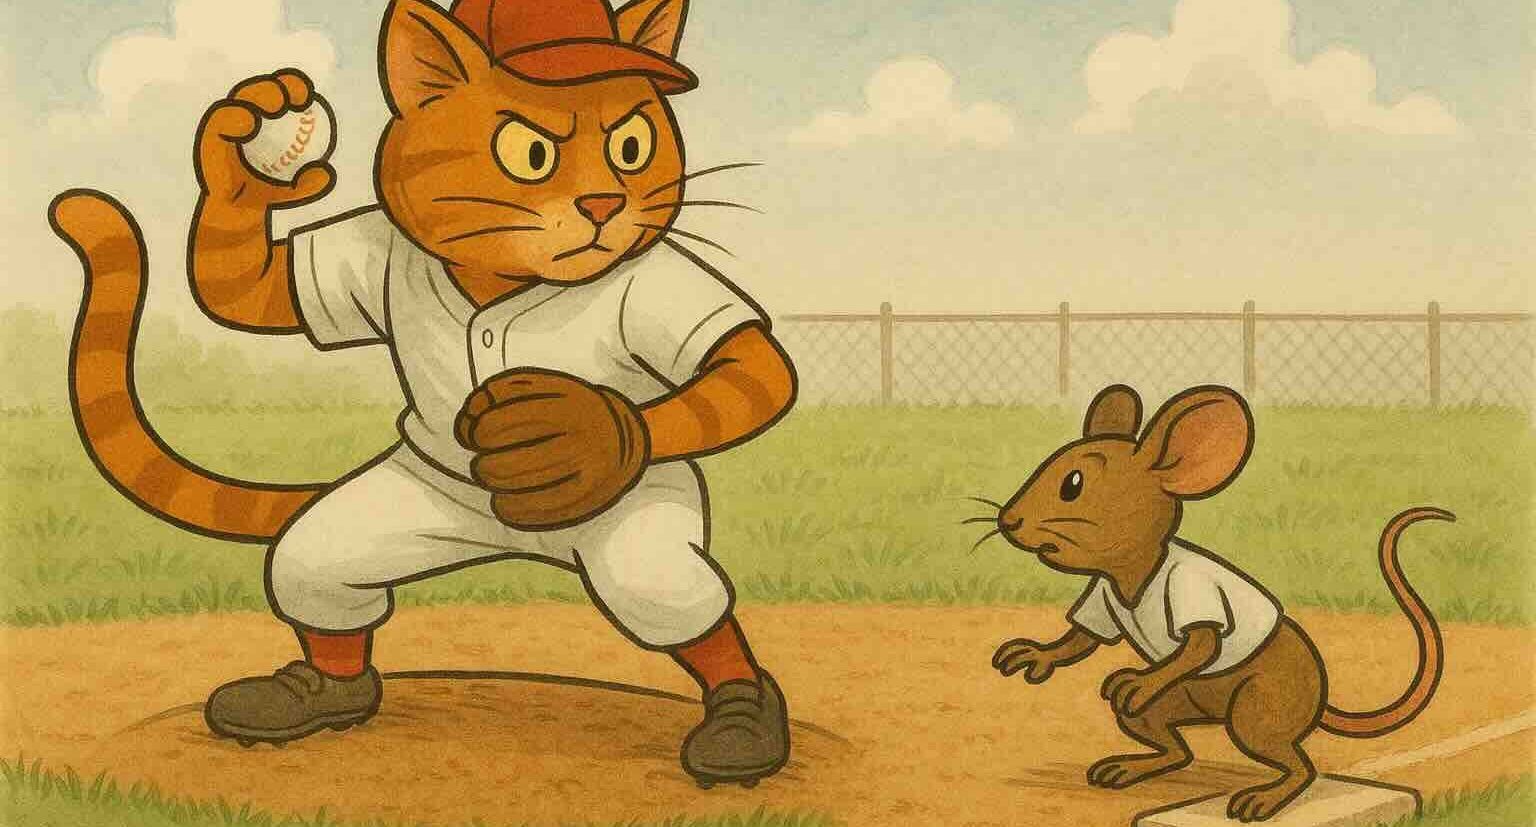
\includegraphics[width = 0.8\textwidth]{images/cat_and_mouse.jpg}
    \begin{itemize}
      \item In 2023, MLB limited the pitcher to 3 pickoff attempts
      \item After 3 failed pickoffs, the runner advances automatically
    \end{itemize}
  \end{frame}

  \begin{frame}{The Puzzle}
    If you are the runner, how much should you extend your lead after each pickoff attempt?\\
    \vfill
    Data: pitch-by-pitch lead distance (player tracking) from MLB*\\
    \vfill
    \footnotesize \it *Major League Baseball trademarks and copyrights are used with permission of MLB Advanced Media, L.P. All rights reserved.
  \end{frame}

  \begin{frame}{Our Approach}
    Step 1: Estimate the effect of lead distance\\
    \begin{itemize}
      \item Linear mixed-effects models (LMMs) for probabilities of pickoff attempt, pickoff success, stolen base success
    \end{itemize}
    ~\\
    Step 2: Solve for the optimal lead distance\\
    \begin{itemize}
      \item Single-player MDP, or two-player stochastic game
%      \item State space: disengagements, bases occupied, outs, count
%      \item Action space: lead distance
%      \item Reward function: runs scored
    \end{itemize}
  \end{frame}

  \begin{frame}{Pickoff Attempt and Success Probability}
    \centering
    \includegraphics[width = 0.45\textwidth]{figures/prob_po_attempt_dark.pdf}
    \hfill
    \includegraphics[width = 0.45\textwidth]{figures/prob_po_success_dark.pdf}
    \begin{itemize}
      \item Fixed effects: \alert{lead distance}, \alert{disengagements}, outs, count, runner sprint speed, catcher arm strength
      \item Random effects: runner, catcher, \alert{pitcher}
    \end{itemize}
  \end{frame}

  \begin{frame}{Stolen Base Success Probability}
    \centering
    \includegraphics[width = 0.9\textwidth]{figures/prob_sb_success_dark.pdf}
    \begin{itemize}
      \item Fixed effects: \alert{lead distance}, disengagements, outs, count, runner sprint speed, catcher arm strength
      \item Random effects: \alert{runner}, catcher, pitcher
    \end{itemize}
  \end{frame}

  \begin{frame}{Runner and Catcher Effects}
    \centering
    \includegraphics[width = 0.45\textwidth]{figures/effect_runner_dark.pdf}
    \hfill
    \includegraphics[width = 0.45\textwidth]{figures/effect_catcher_dark.pdf}
    \begin{itemize}
      \item Fixed effects: lead distance, disengagements, outs, count, \alert{runner sprint speed}, \alert{catcher arm strength}
      \item Random effects: \alert{runner}, \alert{catcher}, pitcher
    \end{itemize}
  \end{frame}

  \begin{frame}{Solving for Optimal Lead Distance}
    Two options:\\
    ~\\
    \begin{enumerate}
      \item Single-player Markov decision process (MDP)
      \begin{itemize}
        \item Runner chooses lead distance
        \item Pitcher follows known stochastic response (no agency)
      \end{itemize}
      ~\\
      \item Two-player stochastic game
      \begin{itemize}
        \item Runner chooses lead distance
        \item Pitcher chooses whether to attempt pickoff
      \end{itemize}
    \end{enumerate}
  \end{frame}

  \begin{frame}{Optimal Lead Distance (single-player MDP)}
    \begin{columns}
      \begin{column}{0.5\textwidth}
        \centering
        \begin{tabular}{c|rrr}
          & \multicolumn{3}{c}{Disengagements}\\
          Count & 1 & 2 & 3\\
          \hline
          0-0 & 10.0 & 11.5 & 14.1 \\ 
          1-0 & 10.2 & 11.7 & 14.2 \\ 
          2-0 & 10.2 & 11.7 & 14.2 \\ 
          3-0 & 10.3 & 11.8 & 14.2 \\ 
          \hline
          0-1 & 9.8 & 11.4 & 14.1 \\ 
          1-1 & 10.0 & 11.6 & 14.2 \\ 
          2-1 & 10.3 & 11.8 & 14.3 \\ 
          3-1 & 10.4 & 11.9 & 14.3 \\ 
          \hline
          0-2 & 9.5 & 11.1 & 14.1 \\ 
          1-2 & 9.9 & 11.4 & 14.3 \\ 
          2-2 & 10.0 & 11.5 & 14.2 \\ 
          3-2 & 10.4 & 11.9 & 14.4
        \end{tabular}
      \end{column}
      \begin{column}{0.5\textwidth}
        \begin{itemize}
          \item \alert{The Two-Foot Rule:} Increase lead by two feet after each disengagement\\
          ~\\
          \item Value of implementation: $\sim$17 runs / team / season ($\sim$\$17,000,000)
        \end{itemize}
      \end{column}
    \end{columns}
  \end{frame}

  \begin{frame}{Optimal Lead Distance (two-player stochastic game)}
    \begin{columns}
      \begin{column}{0.5\textwidth}
        \centering
        \begin{tabular}{c|rrr}
          & \multicolumn{3}{c}{Disengagements}\\
          Count & 1 & 2 & 3\\
          \hline
          0-0 & 11.2 & 11.8 & 16.2 \\ 
          1-0 & 11.2 & 12.0 & 16.1 \\ 
          2-0 & 11.0 & 12.2 & 15.9 \\ 
          3-0 & 10.4 & 11.6 & 15.3 \\ 
          \hline
          0-1 & 10.8 & 11.3 & 16.2 \\ 
          1-1 & 10.9 & 11.1 & 16.1 \\ 
          2-1 & 11.0 & 12.1 & 15.9 \\ 
          3-1 & 10.5 & 11.6 & 15.7 \\ 
          \hline
          0-2 & 10.2 & 10.8 & 16.2 \\ 
          1-2 & 10.5 & 10.4 & 16.3 \\ 
          2-2 & 10.4 & 11.4 & 15.9 \\ 
          3-2 & 10.3 & 11.1 & 15.6 \\ 
        \end{tabular}
      \end{column}
      \begin{column}{0.5\textwidth}
        \begin{itemize}
          \item Equilibrium entails more aggressive behavior from both runner and pitcher\\
        \end{itemize}
      \end{column}
    \end{columns}
  \end{frame}

  \begin{frame}
    \Large Part II: Pitcher evaluation from pitch tracking\normalsize\\
    \vfill
    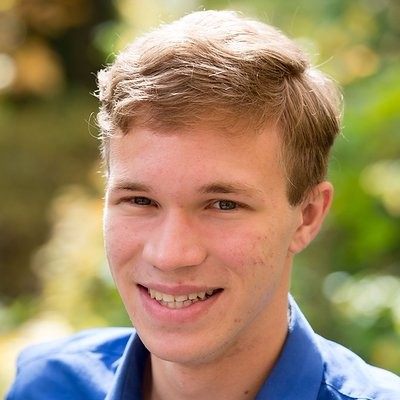
\includegraphics[height=0.5in]{images/collaborators/iglesias.jpg}
    \alert{Vicente Iglesias}, Susquehanna International Group\\
    ~\\
    Working paper:\\
    \small Powers S, Iglesias V ``Pitch trajectory density estimation for predicting future outcomes''
  \end{frame}

  \begin{frame}{Background}
    \begin{center}
      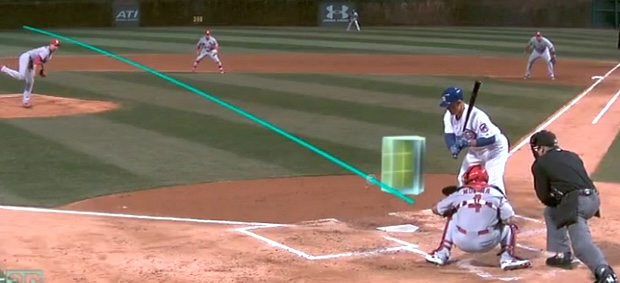
\includegraphics[width = 0.8\textwidth]{images/pitch_tracking.jpg}
    \end{center}
    \begin{itemize}
      \item Full pitch tracking data have been available for two decades
      \item Trajectory estimated as 3D quadratic function of time ($\in \mathbb{R}^9$)
      \item Standard practice: Evaluate pitchers based on trajectories
    \end{itemize}
  \end{frame}

  \begin{frame}{The Puzzle}
    \begin{columns}
      \begin{column}{0.5\textwidth}
        \centering
        $\mbox{Variable Importance}^1$\\
        \includegraphics[width = \textwidth]{figures/feature_importance_dark.pdf}
      \end{column}
      \begin{column}{0.5\textwidth}
        \centering
        $\mbox{Variable Reliability}^2$\\
        \includegraphics[width = \textwidth]{figures/feature_reliability_dark.pdf}
      \end{column}
    \end{columns}
    \scriptsize
    \vfill
    ${}^1$ fractional contribution of each feature's splits to gradient boosting pitch model\\
    ${}^2$ (between-pitcher variance) / (total variance); varies by pitch type (here: RHB FB)
  \end{frame}

  \begin{frame}{Why Supervised Learning Isn't Enough}
    \begin{columns}
      \begin{column}{0.4\columnwidth}
        \centering
        {\bf Supervised Learning}\\
        ~\\
        \begin{tabular}{ccc}
          Pitch &               & Outcome\\
          $x_1$ & $\rightarrow$ & $y_1$\\
          $x_2$ & $\rightarrow$ & $y_2$\\
          $x_3$ & $\rightarrow$ & $y_3$\\
                & ...           &      \\
          $x_n$ & $\rightarrow$ & $y_n$\\
          \\
          \\
          \\
          $x^*$ & $\rightarrow$ & $\hat y = \hat f(x)$\\
        \end{tabular}
      \end{column}
      \begin{column}{0.6\columnwidth}
        \centering
        {\bf Our Problem}\\
        ~\\
        \begin{tabular}{cccc}
          Pitcher & Pitch &               & Outcome\\
          A       & $x_1$ & $\rightarrow$ & $y_1$\\
          A       & $x_2$ & $\rightarrow$ & $y_2$\\
          B       & $x_3$ & $\rightarrow$ & $y_3$\\
                  &       & ...           &      \\
          C       & $x_n$ & $\rightarrow$ & $y_n$\\
                  & \\
                  &       & $\searrow$    & {\color{solarizedRebase03} $\int\hat p(x)\hat f(x)$}\\
                  & \\
          A       &  {\color{solarizedRebase03} $\hat p(x|\text{A})$}     &               & $\hat y$\\
        \end{tabular}
      \end{column}
    \end{columns}
  \end{frame}

  \begin{frame}{Why Supervised Learning Isn't Enough}
    \begin{columns}
      \begin{column}{0.4\columnwidth}
        \centering
        {\bf Supervised Learning}\\
        ~\\
        \begin{tabular}{ccc}
          Pitch &               & Outcome\\
          $x_1$ & $\rightarrow$ & $y_1$\\
          $x_2$ & $\rightarrow$ & $y_2$\\
          $x_3$ & $\rightarrow$ & $y_3$\\
                & ...           &      \\
          $x_n$ & $\rightarrow$ & $y_n$\\
          \\
          \\
          \\
          $x^*$ & $\rightarrow$ & $\hat y = \hat f(x)$\\
        \end{tabular}
      \end{column}
      \begin{column}{0.6\columnwidth}
        \centering
        \alert{\bf Our Approach}\\
        ~\\
        \begin{tabular}{cccc}
          Pitcher & Pitch &               & Outcome\\
          A       & $x_1$ & $\rightarrow$ & $y_1$\\
          A       & $x_2$ & $\rightarrow$ & $y_2$\\
          B       & $x_3$ & $\rightarrow$ & $y_3$\\
                  &       & ...           &      \\
          C       & $x_n$ & $\rightarrow$ & $y_n$\\
                  & \\
                  & \alert{$\downarrow$}\\
                  & \\
          A       & \alert{$\hat p(x|\text{A})$} & \alert{$\rightarrow$} & \alert{$\int\hat p(x)\hat f(x)$}\\
        \end{tabular}
      \end{column}
    \end{columns}
  \end{frame}

  \begin{frame}{Our Approach}
    Step 1: Estimate trajectory distributions conditional on covariates\\
    \begin{itemize}
      \item Bayesian hierarchical model (9D MVN likelihood)
%      \item Mean $\sim$ pitcher, context, pitcher $\times$ context
%      \item Variance scaling $\sim$ pitcher, context
%      \item Correlation $\sim$ pitcher
%      \item Fit via maximum {\it a posteriori} (MAP) estimator
    \end{itemize}
    ~\\
    Step 2: Fit supervised learning model and integrate w.r.t. Step 1\\
    \begin{itemize}
      \item Gradient boosting
    \end{itemize}
  \end{frame}

  \begin{frame}{Dylan Cease's Slider vs RHB in 0-0 Counts}
    \begin{columns}
      \begin{column}{0.5\textwidth}
        \centering
        Predicted Break Chart\\
        ~\\
        
\includegraphics[width = 0.9\textwidth]{figures/656302_SL_R_0_0_break.png}
      \end{column}
      \begin{column}{0.5\textwidth}
        \centering
        Predicted Plate Location\\
        ~\\
        
\includegraphics[width = 0.9\textwidth]{figures/656302_SL_R_0_0_plate.png}
      \end{column}
    \end{columns}
  \end{frame}

  \begin{frame}{Dylan Cease's Slider vs RHB in All Counts}
    \centering
    
\includegraphics[height = 0.85\textheight]{figures/656302_SL_R_plate.png}
  \end{frame}

  \begin{frame}{Predictive Performance}
    \centering
    
\includegraphics[width = \textwidth]{figures/cor_by_sample_size.pdf}
  \end{frame}

  \begin{frame}
    \Large Part III: Inference from swing-level bat tracking \normalsize\\
    \vfill
    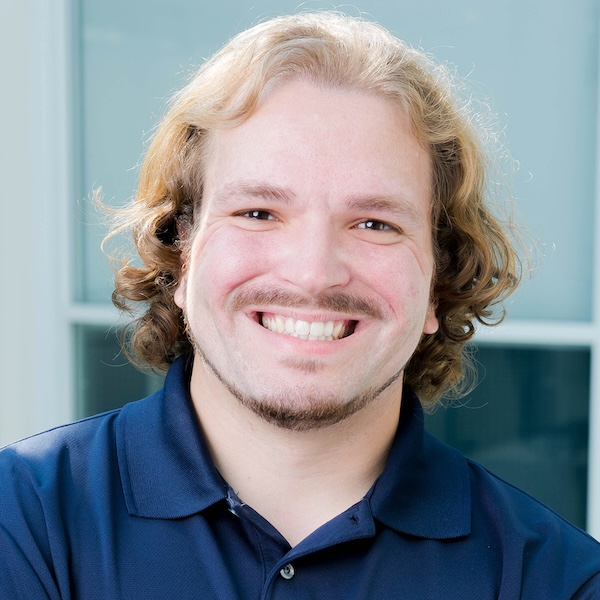
\includegraphics[height=0.5in]{images/collaborators/yurko.jpg}
    \alert{Ron Yurko}, Carnegie Mellon University\\
    ~\\
    Working paper:\\
    \small Powers S, Yurko R ``Swinging, Fast and Slow: Interpreting variation in baseball swing tracking metrics'' arXiv:2507.01238
  \end{frame}

  \begin{frame}{Background}
    \begin{center}
      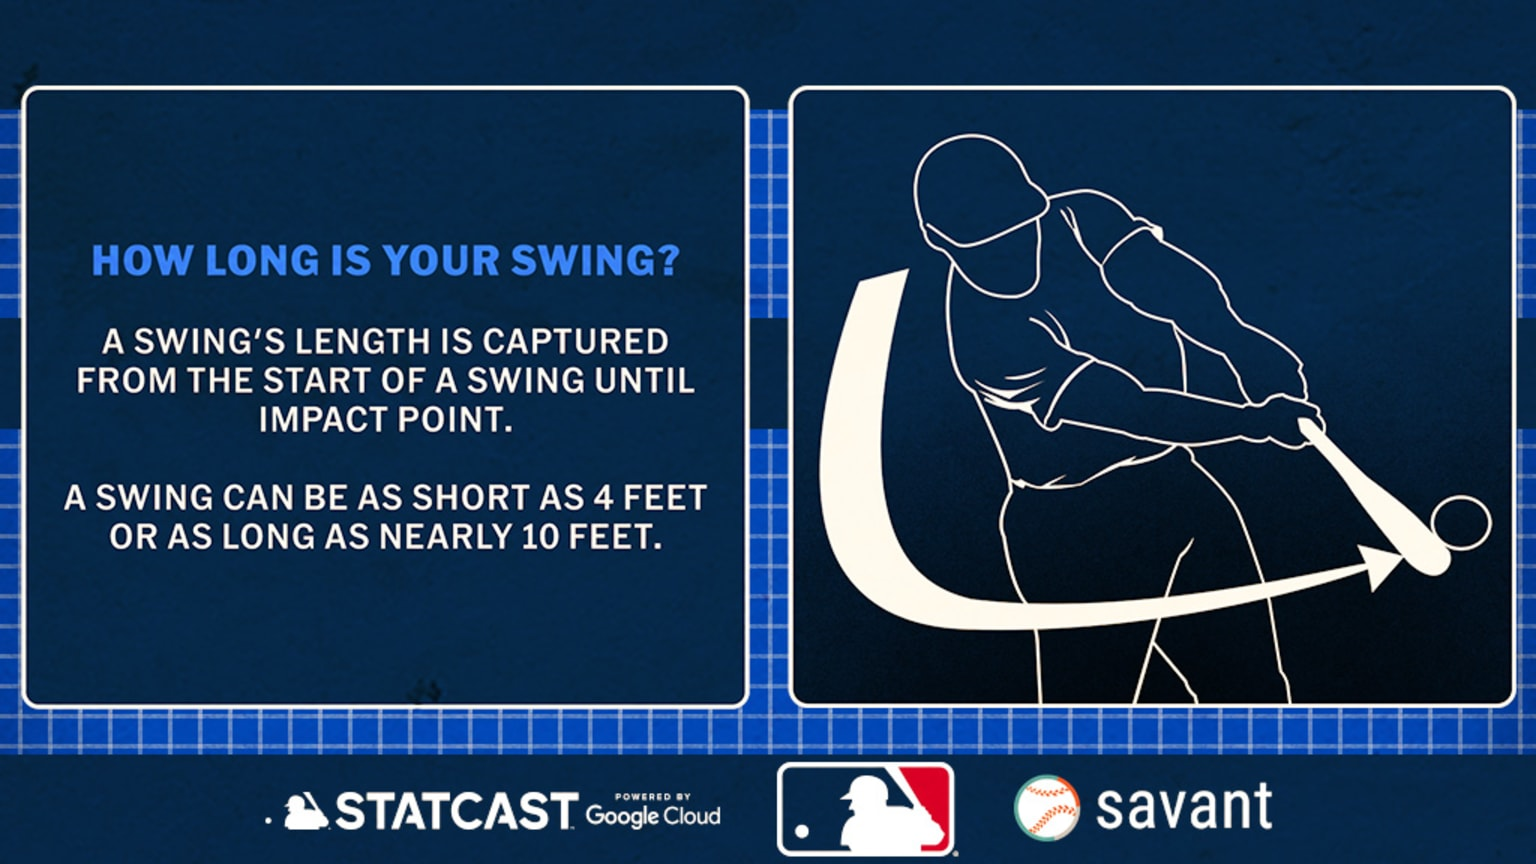
\includegraphics[width = 0.8\textwidth]{images/swing_length.jpg}
    \end{center}
    \begin{itemize}
      \item In May 2024, MLB released swing length and bat speed data
      \item Both are measured at contact (or at point nearest to contact)
    \end{itemize}
  \end{frame}

  \begin{frame}{The Puzzle}
    \begin{center}
      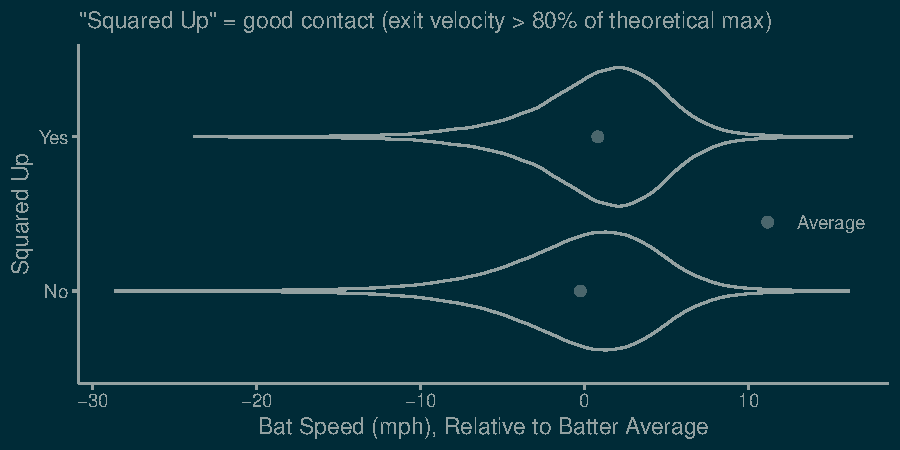
\includegraphics[width = \textwidth]{figures/counterintuitive.pdf}
    \end{center}
    \begin{itemize}
      \item How should batters modulate swing length and bat speed?
    \end{itemize}
  \end{frame}

  \begin{frame}{Challenge \#1: Measurement}
    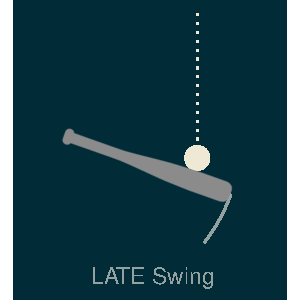
\includegraphics[width = 0.49\textwidth]{figures/swing_late.pdf}
    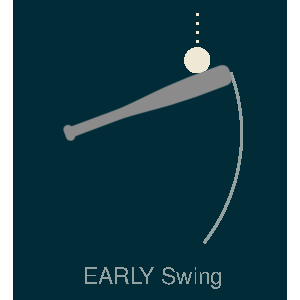
\includegraphics[width = 0.49\textwidth]{figures/swing_early.pdf}
    \begin{itemize}
      \item For \alert{identical} swings, timing determines point of measurement
      \item Swing length and bat speed are \alert{outcomes}, not purely process
    \end{itemize}
  \end{frame}

  \begin{frame}{Challenge \#2: Confounding}
    \begin{center}
      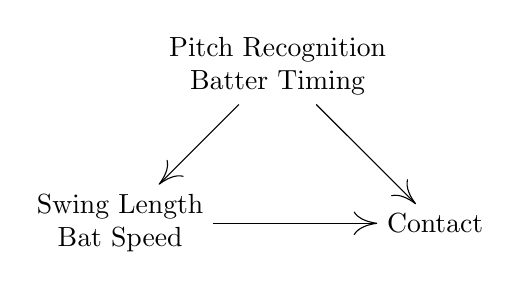
\begin{tikzpicture}[->, align = center]
        \node (confounders) at (2, 2) {Pitch Recognition \\ Batter Timing};
        \node (swing_metrics) at (0, 0) {Swing Length \\ Bat Speed};
        \node (contact) at (4, 0) {Contact};
        \draw (confounders) -- (swing_metrics);
        \draw (confounders) -- (contact);
        \draw (swing_metrics) -- (contact);
      \end{tikzpicture}
    \end{center}
  \end{frame}

  \begin{frame}{Our Approach}
    Step 1: Estimate batter intention\\
    \begin{itemize}
      \item Bayesian hierarchical model (skew-normal likelihood)
      \item Condition on successful contact against fastballs!
%      \item Skew $\sim$ batter
    \end{itemize}
    ~\\
    Step 2: Estimate effect of batter intention\\
    \begin{itemize}
      \item Instrumental variable regression (instrument: count)
    \end{itemize}
  \end{frame}

  \begin{frame}{Batter $\times$ Count Interaction}
    \centering
    \includegraphics[height = 0.7\textheight]{figures/approach_dark.pdf}
    \begin{itemize}
      \item Effects: \alert{batter}, count, location, \alert{batter} $\times$ (\alert{count}, location)
      \item We observe heterogeneity in how batters adjust to count
    \end{itemize}
  \end{frame}

  \begin{frame}{Causal Effect Estimates}
    \includegraphics[width = 0.49\textwidth]{figures/bat_speed_contact_dark.pdf}
    \includegraphics[width = 0.49\textwidth]{figures/bat_speed_power_dark.pdf}
    \begin{itemize}
      \item Batters who slow down more with two strikes exhibit\\ \alert{more contact} (relative to expectation) with two strikes
      \item Batters who slow down more with two strikes exhibit\\ \alert{less power} (relative to expectation) with two strikes
      \item Is the tradeoff worthwhile?
    \end{itemize}
  \end{frame}

  \begin{frame}{Contact-Power Tradeoff}
    \centering
    \includegraphics[height = 0.7\textheight]{figures/approach_run_value_dark.pdf}
    \begin{itemize}
      \item Batters can reduce strikeouts by slowing their bat speeds,\\ but the tradeoff in power makes it a wash
    \end{itemize}
  \end{frame}

  \begin{frame}{Thank You!}
    \centering saberpowers.github.io
  \end{frame}

\end{document}
